\chapter{Example Application 1}\label{chapter:poc1}

\section{Introduction}
Existing applications for sharing files are central solutions and therefore suffer from single point of failure risk. Moreover, using central services for securing data means that we have to trust a 3rd party with our data thus exposing it to manipulation risks. Hence, a decentralized
application is required to overcome the problems posed by a central application. With the recent developments in Blockchain technology and P2P storage, it is possible to securely store and share data without using any central server.

This chapter describes the workings of the application \textit{dShare}\cite{harsh_kedia_2019_3359852} built using P2P technologies enabling a secure way of storing and sharing data between two individuals or entities. The latest version of the application is deployed at \url{https://file-share-dapp.herokuapp.com/}

\section{Technologies Used}

\subsection{Ethereum}
Ethereum\cite{buterin2014ethereum} is a blockchain platform for building decentralized applications. It allows the creation of \textit{Smart Contracts}. Solidity\footnote{\url{https://github.com/ethereum/solidity}} is the primary language for writing smart contracts on Ethereum.

\subsection{InterPlanetary File System (IPFS)}
IPFS\cite{benet2014ipfs} is a peer-to-peer file transfer protocol which enables a shared file system between all its connected peers. It achieves this by combining previous peer-to-peer systems such as Distributed Hash Tables (DHT), BitTorrent\cite{cohen2008bittorrent}, and Git\cite{loeliger2012version}. The data in the IPFS network are modeled as a Merkle DAG\footnote{Merkle directed acyclic graph - similiar to a Merkle tree data structure however they do not need to be balanced and it’s non-leaf nodes can contain some data.} thus providing a throughput storage system with content-addressed hyperlinks.

\subsection{OriginStamp}
OriginStamp\cite{hepp2018originstamp} is a blockchain based system for decentralized timestamping. It uses the Bitcoin blockchain for the creation of trusted and immutable timestamps for any piece of data. Timestamps created by OriginStamp can be verified independently by anyone.

\begin{figure}[h]
	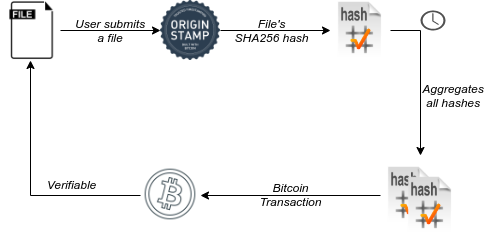
\includegraphics[width=\linewidth]{figures/origin-stamp}
	\caption{\label{fig:originstamp} Timestamping using OriginStamp}
\end{figure}

Figure~\ref{fig:originstamp} visualizes the timestamping process as implemented in OriginStamp. When a user submits a file, the hash of the data is recorded. It combines all the hashes submitted over a period of time and generates an aggregated hash. After some additional hashing and encoding operations, a Bitcoin address is created to which the smallest possible transactional amount of Bitcoins is transferred. Performing this transaction embeds the hash and the timestamp permanently to the Bitcoin blockchain. Each transaction is part of a block and is added to the Bitcoin blockchain by a process called mining. Since each block is linked cryptographically to the previous block, adding a new block confirms the validity of the last block. Changing the timestamp of a transaction becomes impossible once five or six subsequent blocks are mined, which requires an hour on average\cite{nakamoto2008bitcoin}.

\section{Implementation}
For storing of files we used IPFS. Before uploading to the IPFS network, files are encrypted using AES-GCM\footnote{\url{https://www.aes-gcm.com/}} encryption mechanism. Sharing of encryption keys is facilitated using smart contracts built on Ethereum; thus files can be shared by anyone with an Ethereum address. Finally, OriginStamp is used for immutable timestamping.

The front-end of the application is built using React.js\footnote{\url{https://reactjs.org/}}, a JavaScript library for building user interfaces. Solidity was used for writing smart contracts and deployed on the Ethereum test network, Rinkeby\footnote{\url{https://www.rinkeby.io}}. Next.js\footnote{\url{https://nextjs.org/}} was used for server-side rendering (SSR)\footnote{\url{https://nextjs.org/features/server-side-rendering/}}, and Firebase\footnote{\url{https://firebase.google.com/}} was used as a database for storing public Ethereum key of the users.

\section{Working}
This section describes the working of the different components of the application.

\subsection{Smart Contract}
The smart contract serves as the bridge between the front-end of the application and the Ethereum Blockchain. Data is read from and written to the blockchain with the help of function calls in the contract. Each function call which modifies some data requires a small fee in the form of gas\footnote{\url{https://ethereum.stackexchange.com/questions/3/what-is-meant-by-the-term-gas}} which defines the cost for a function execution in Ether. Reading from the blockchain does not require any fees.

The application makes use of two contracts, \textit{FileFactory}, which acts as the factory contract for creation of new files and \textit{File}, which represents an individual file.

\subsubsection{FileFactory}
\textit{FileFactory} is the contract which is deployed on the Rinkeby test network. It has several mappings which stores the list of file contracts uploaded by a user. Whenever a user uploads a file, a function call is made to the \textit{FileFactory} contract, which in turn deploys the \textit{File} contract and updates the mappings for list of uploaded files and the respective uploader.

\subsubsection{File}
File contract is deployed to the blockchain whenever a file is successfully uploaded to the IPFS network using the application. Upon deployed, the constructor function is called. It takes the values passed by the \textit{FileFactory} contract and saves the details to it’s \textit{File} contract.

\subsection{File Upload}
Figure~\ref{fig:ethereum-upload} visualizes the working of the application when a user uploads a file.

\begin{figure}[h]
	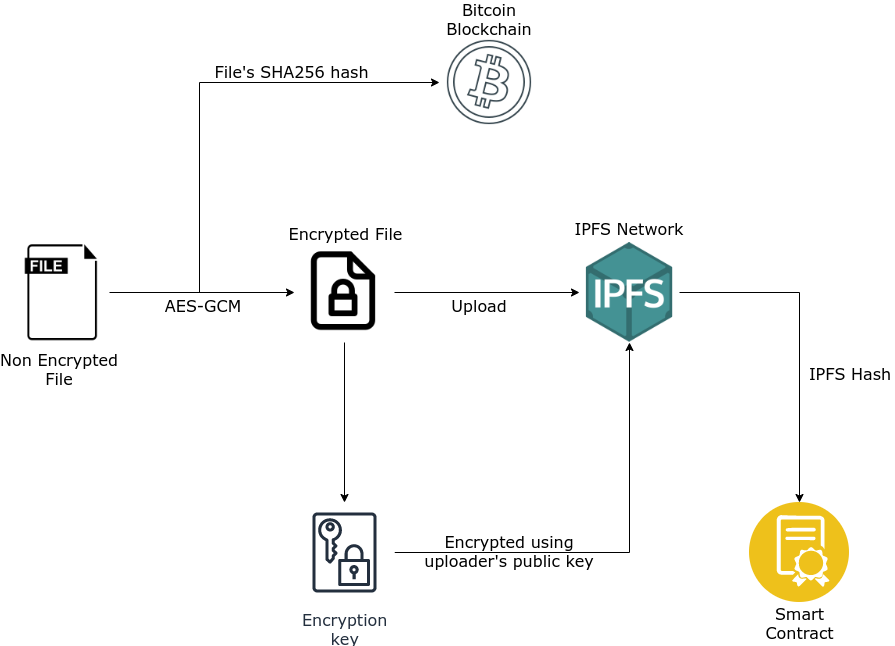
\includegraphics[width=\linewidth]{figures/ethereum-upload}
	\caption{\label{fig:ethereum-upload} File Upload using Ethereum dApp}
\end{figure}

As soon as a user submits a file to be uploaded, it's SHA-256\footnote{\url{https://www.movable-type.co.uk/scripts/sha256.html}} hash is calculated and a timestamp is created by submitting the hash to the bitcoin blockchain using the OriginStamp API\footnote{\url{http://doc.originstamp.org/}}.

Next, the file is encrypted using the SubtleCrypto\footnote{\url{https://developer.mozilla.org/en-US/docs/Web/API/SubtleCrypto}} interface with 'AES-GCM'\footnote{\url{https://en.wikipedia.org/wiki/Galois/Counter_Mode}} as the encrypting algorithm. The encrypted data is then combined with the random salt to generate a \texttt{Uint8Array} buffer ready to be uploaded to the IPFS network.

The key used to encrypt the file is converted to \texttt{JSON} and is encrypted using the uploader's Ethereum public key which is retrieved from the database. This encrypted key and the encrypted data is then uploaded to the IPFS network. Once the file is successfully uploaded, \texttt{createFile()} in the \texttt{FileFactory} contract is called which deploys a new \texttt{File} contract with all details regarding the file saved to the blockchain.

\subsection{File Sharing}
Sharing a file requires the recipient's Ethereum address and uploader's private key. Figure~\ref{fig:ethereum-share} visualizes the working of the application when a user shares a file with another user.

\begin{figure}[h]
	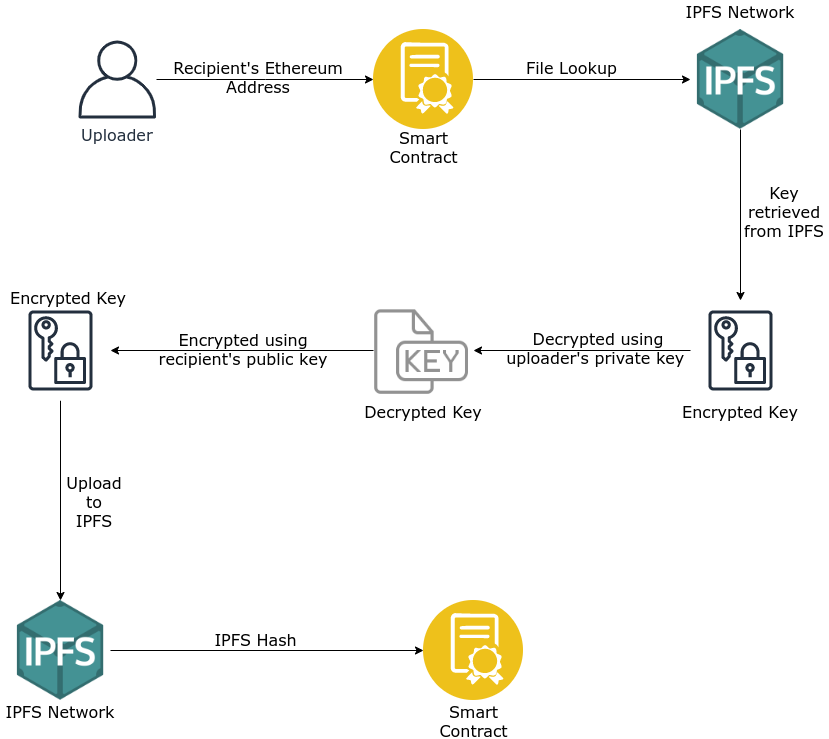
\includegraphics[width=\linewidth]{figures/ethereum-share}
	\caption{\label{fig:ethereum-share} File Sharing using Ethereum dApp}
\end{figure}

Firstly, the file's IPFS location is retrieved from the \texttt{File} contract. From this location, the encrypted key is download and decrypted using uploader's private key. Once decrypted, the key is again encrypted using a recipient's public key. The new encrypted key is again uploaded to the IPFS network. Finally, the IPFS location of the key is saved into the \texttt{File} contract by calling \texttt{shareFile()}.

To stop sharing a file, a function call can be made to the \texttt{File} contract with the recipient's address, which deletes the contract reference from the \texttt{recipientFiles} array.

\subsection{File Download}
Downloading a file requires the user's Ethereum private key. Depending on whether the file is uploaded or shared one, corresponding function from the \texttt{File} contract is called to retrieve the file's details. The key is then decrypted using user's private key and is converted to a valid JSON web key (jwk)\footnote{\url{https://tools.ietf.org/html/rfc7517}} format. The encrypted file data is then converted to a file buffer, and the original file content and the random salt used for encrypting the file is retrieved. Finally, the file is decrypted and saved to the user's local storage.

\subsection{File Archiving}
Instead of deleting a \texttt{File} contract, the application provides a way to achieve files. This is also useful to keep track of archived files and restore them at a later date if required. When a file is archived, the \texttt{File} contract address is saved in an array which is later used for filtering the archived files from the UI. Restoring a file removes the \texttt{File} contract address from the archived files array.